\documentclass[1p]{elsarticle_modified}
%\bibliographystyle{elsarticle-num}

%\usepackage[colorlinks]{hyperref}
%\usepackage{abbrmath_seonhwa} %\Abb, \Ascr, \Acal ,\Abf, \Afrak
\usepackage{amsfonts}
\usepackage{amssymb}
\usepackage{amsmath}
\usepackage{amsthm}
\usepackage{scalefnt}
\usepackage{amsbsy}
\usepackage{kotex}
\usepackage{caption}
\usepackage{subfig}
\usepackage{color}
\usepackage{graphicx}
\usepackage{xcolor} %% white, black, red, green, blue, cyan, magenta, yellow
\usepackage{float}
\usepackage{setspace}
\usepackage{hyperref}

\usepackage{tikz}
\usetikzlibrary{arrows}

\usepackage{multirow}
\usepackage{array} % fixed length table
\usepackage{hhline}

%%%%%%%%%%%%%%%%%%%%%
\makeatletter
\renewcommand*\env@matrix[1][\arraystretch]{%
	\edef\arraystretch{#1}%
	\hskip -\arraycolsep
	\let\@ifnextchar\new@ifnextchar
	\array{*\c@MaxMatrixCols c}}
\makeatother %https://tex.stackexchange.com/questions/14071/how-can-i-increase-the-line-spacing-in-a-matrix
%%%%%%%%%%%%%%%

\usepackage[normalem]{ulem}

\newcommand{\msout}[1]{\ifmmode\text{\sout{\ensuremath{#1}}}\else\sout{#1}\fi}
%SOURCE: \msout is \stkout macro in https://tex.stackexchange.com/questions/20609/strikeout-in-math-mode

\newcommand{\cancel}[1]{
	\ifmmode
	{\color{red}\msout{#1}}
	\else
	{\color{red}\sout{#1}}
	\fi
}

\newcommand{\add}[1]{
	{\color{blue}\uwave{#1}}
}

\newcommand{\replace}[2]{
	\ifmmode
	{\color{red}\msout{#1}}{\color{blue}\uwave{#2}}
	\else
	{\color{red}\sout{#1}}{\color{blue}\uwave{#2}}
	\fi
}

\newcommand{\Sol}{\mathcal{S}} %segment
\newcommand{\D}{D} %diagram
\newcommand{\A}{\mathcal{A}} %arc


%%%%%%%%%%%%%%%%%%%%%%%%%%%%%5 test

\def\sl{\operatorname{\textup{SL}}(2,\Cbb)}
\def\psl{\operatorname{\textup{PSL}}(2,\Cbb)}
\def\quan{\mkern 1mu \triangleright \mkern 1mu}

\theoremstyle{definition}
\newtheorem{thm}{Theorem}[section]
\newtheorem{prop}[thm]{Proposition}
\newtheorem{lem}[thm]{Lemma}
\newtheorem{ques}[thm]{Question}
\newtheorem{cor}[thm]{Corollary}
\newtheorem{defn}[thm]{Definition}
\newtheorem{exam}[thm]{Example}
\newtheorem{rmk}[thm]{Remark}
\newtheorem{alg}[thm]{Algorithm}

\newcommand{\I}{\sqrt{-1}}
\begin{document}

%\begin{frontmatter}
%
%\title{Boundary parabolic representations of knots up to 8 crossings}
%
%%% Group authors per affiliation:
%\author{Yunhi Cho} 
%\address{Department of Mathematics, University of Seoul, Seoul, Korea}
%\ead{yhcho@uos.ac.kr}
%
%
%\author{Seonhwa Kim} %\fnref{s_kim}}
%\address{Center for Geometry and Physics, Institute for Basic Science, Pohang, 37673, Korea}
%\ead{ryeona17@ibs.re.kr}
%
%\author{Hyuk Kim}
%\address{Department of Mathematical Sciences, Seoul National University, Seoul 08826, Korea}
%\ead{hyukkim@snu.ac.kr}
%
%\author{Seokbeom Yoon}
%\address{Department of Mathematical Sciences, Seoul National University, Seoul, 08826,  Korea}
%\ead{sbyoon15@snu.ac.kr}
%
%\begin{abstract}
%We find all boundary parabolic representation of knots up to 8 crossings.
%
%\end{abstract}
%\begin{keyword}
%    \MSC[2010] 57M25 
%\end{keyword}
%
%\end{frontmatter}

%\linenumbers
%\tableofcontents
%
\newcommand\colored[1]{\textcolor{white}{\rule[-0.35ex]{0.8em}{1.4ex}}\kern-0.8em\color{red} #1}%
%\newcommand\colored[1]{\textcolor{white}{ #1}\kern-2.17ex	\textcolor{white}{ #1}\kern-1.81ex	\textcolor{white}{ #1}\kern-2.15ex\color{red}#1	}

{\Large $\underline{12a_{0011}~(K12a_{0011})}$}

\setlength{\tabcolsep}{10pt}
\renewcommand{\arraystretch}{1.6}
\vspace{1cm}\begin{tabular}{m{100pt}>{\centering\arraybackslash}m{274pt}}
\multirow{5}{120pt}{
	\centering
	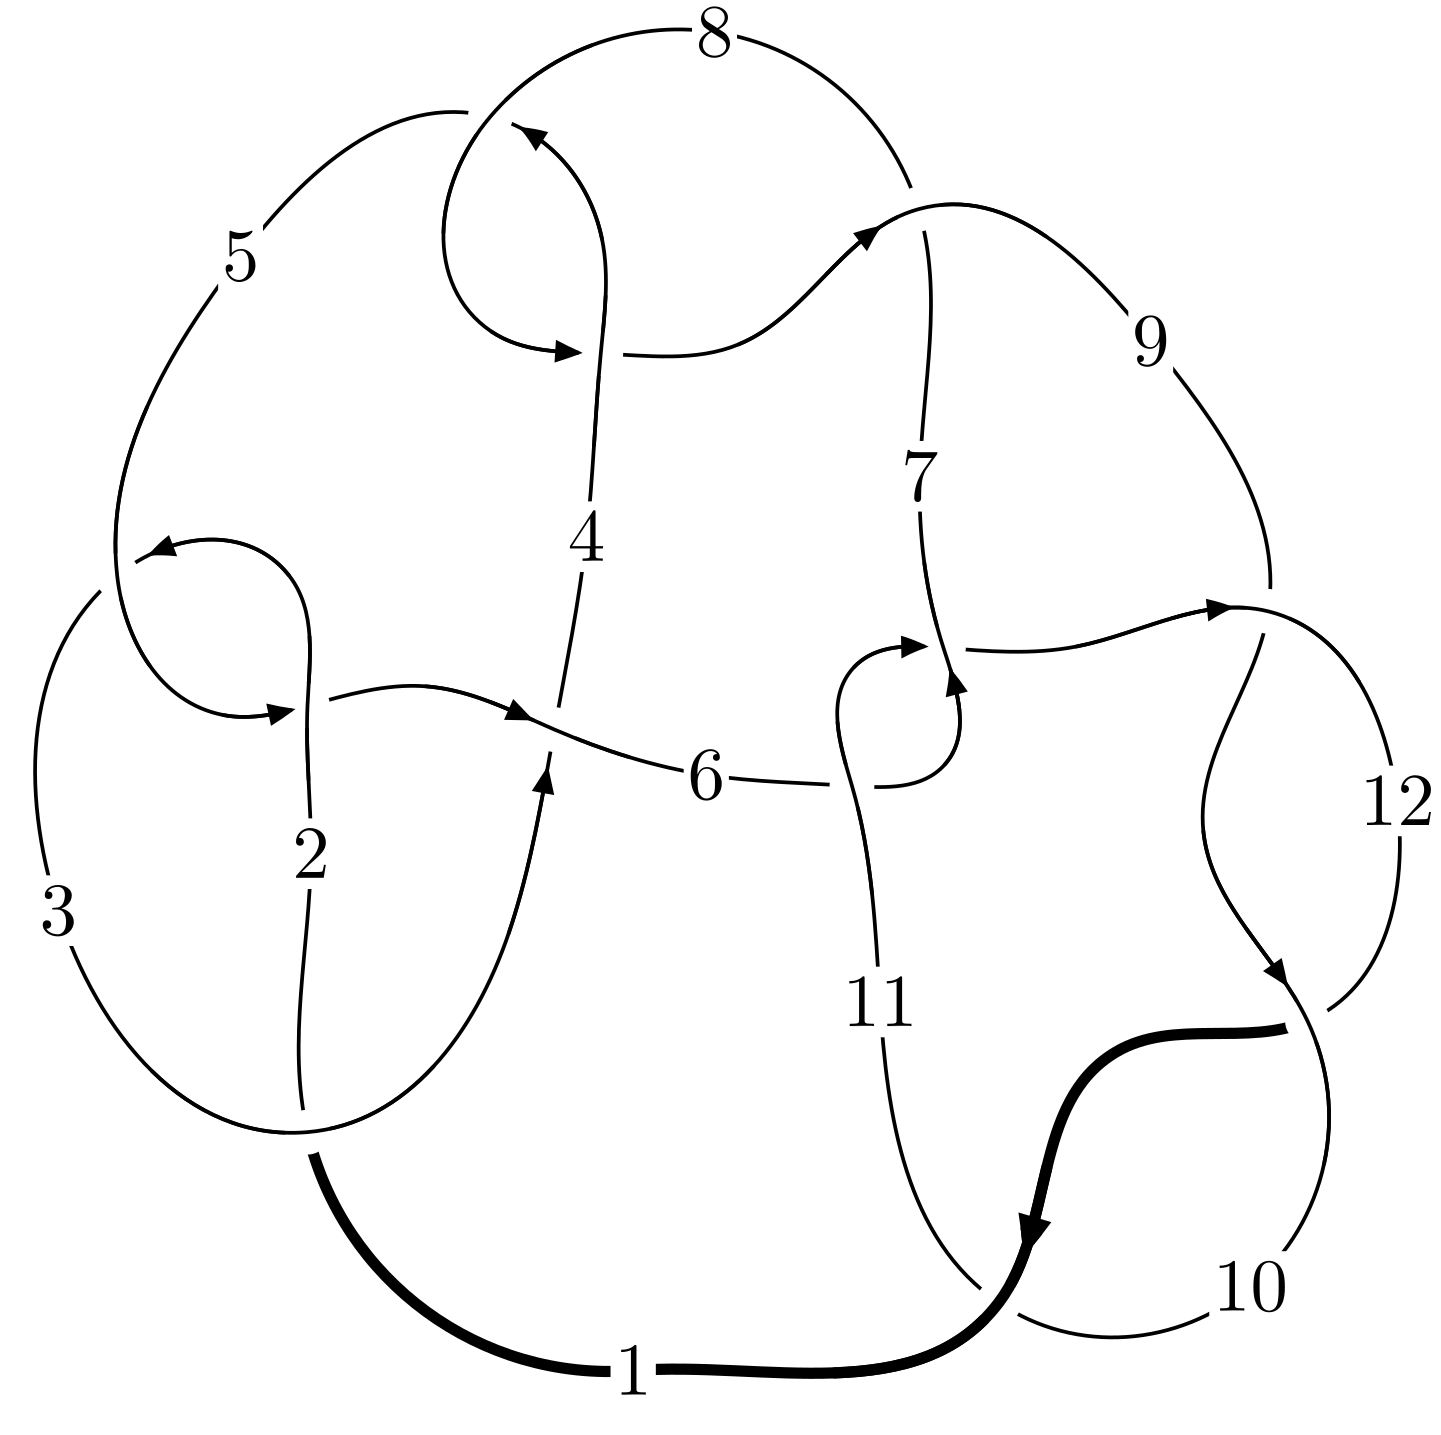
\includegraphics[width=112pt]{../../../GIT/diagram.site/Diagrams/png/812_12a_0011.png}\\
\ \ \ A knot diagram\footnotemark}&
\allowdisplaybreaks
\textbf{Linearized knot diagam} \\
\cline{2-2}
 &
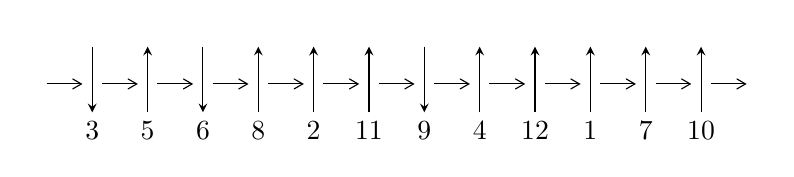
\begin{tikzpicture}[x=20pt, y=17pt]
	% nodes
	\node (C0) at (0, 0) {};
	\node (C1) at (1, 0) {};
	\node (C1U) at (1, +1) {};
	\node (C1D) at (1, -1) {3};

	\node (C2) at (2, 0) {};
	\node (C2U) at (2, +1) {};
	\node (C2D) at (2, -1) {5};

	\node (C3) at (3, 0) {};
	\node (C3U) at (3, +1) {};
	\node (C3D) at (3, -1) {6};

	\node (C4) at (4, 0) {};
	\node (C4U) at (4, +1) {};
	\node (C4D) at (4, -1) {8};

	\node (C5) at (5, 0) {};
	\node (C5U) at (5, +1) {};
	\node (C5D) at (5, -1) {2};

	\node (C6) at (6, 0) {};
	\node (C6U) at (6, +1) {};
	\node (C6D) at (6, -1) {11};

	\node (C7) at (7, 0) {};
	\node (C7U) at (7, +1) {};
	\node (C7D) at (7, -1) {9};

	\node (C8) at (8, 0) {};
	\node (C8U) at (8, +1) {};
	\node (C8D) at (8, -1) {4};

	\node (C9) at (9, 0) {};
	\node (C9U) at (9, +1) {};
	\node (C9D) at (9, -1) {12};

	\node (C10) at (10, 0) {};
	\node (C10U) at (10, +1) {};
	\node (C10D) at (10, -1) {1};

	\node (C11) at (11, 0) {};
	\node (C11U) at (11, +1) {};
	\node (C11D) at (11, -1) {7};

	\node (C12) at (12, 0) {};
	\node (C12U) at (12, +1) {};
	\node (C12D) at (12, -1) {10};
	\node (C13) at (13, 0) {};

	% arrows
	\draw[->,>={angle 60}]
	(C0) edge (C1) (C1) edge (C2) (C2) edge (C3) (C3) edge (C4) (C4) edge (C5) (C5) edge (C6) (C6) edge (C7) (C7) edge (C8) (C8) edge (C9) (C9) edge (C10) (C10) edge (C11) (C11) edge (C12) (C12) edge (C13) ;	\draw[->,>=stealth]
	(C1U) edge (C1D) (C2D) edge (C2U) (C3U) edge (C3D) (C4D) edge (C4U) (C5D) edge (C5U) (C6D) edge (C6U) (C7U) edge (C7D) (C8D) edge (C8U) (C9D) edge (C9U) (C10D) edge (C10U) (C11D) edge (C11U) (C12D) edge (C12U) ;
	\end{tikzpicture} \\
\hhline{~~} \\& 
\textbf{Solving Sequence} \\ \cline{2-2} 
 &
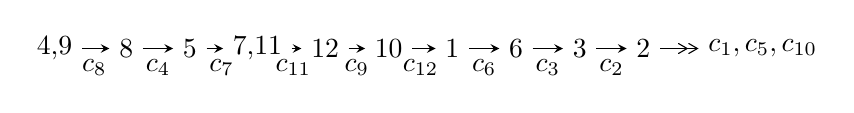
\begin{tikzpicture}[x=23pt, y=7pt]
	% node
	\node (A0) at (-1/8, 0) {4,9};
	\node (A1) at (1, 0) {8};
	\node (A2) at (2, 0) {5};
	\node (A3) at (49/16, 0) {7,11};
	\node (A4) at (33/8, 0) {12};
	\node (A5) at (41/8, 0) {10};
	\node (A6) at (49/8, 0) {1};
	\node (A7) at (57/8, 0) {6};
	\node (A8) at (65/8, 0) {3};
	\node (A9) at (73/8, 0) {2};
	\node (C1) at (1/2, -1) {$c_{8}$};
	\node (C2) at (3/2, -1) {$c_{4}$};
	\node (C3) at (5/2, -1) {$c_{7}$};
	\node (C4) at (29/8, -1) {$c_{11}$};
	\node (C5) at (37/8, -1) {$c_{9}$};
	\node (C6) at (45/8, -1) {$c_{12}$};
	\node (C7) at (53/8, -1) {$c_{6}$};
	\node (C8) at (61/8, -1) {$c_{3}$};
	\node (C9) at (69/8, -1) {$c_{2}$};
	\node (A10) at (11, 0) {$c_{1},c_{5},c_{10}$};

	% edge
	\draw[->,>=stealth]	
	(A0) edge (A1) (A1) edge (A2) (A2) edge (A3) (A3) edge (A4) (A4) edge (A5) (A5) edge (A6) (A6) edge (A7) (A7) edge (A8) (A8) edge (A9) ;
	\draw[->>,>={angle 60}]	
	(A9) edge (A10);
\end{tikzpicture} \\ 

\end{tabular} \\

\footnotetext{
The image of knot diagram is generated by the software ``\textbf{Draw programme}" developed by Andrew Bartholomew(\url{http://www.layer8.co.uk/maths/draw/index.htm\#Running-draw}), where we modified some parts for our purpose(\url{https://github.com/CATsTAILs/LinksPainter}).
}\phantom \\ \newline 
\centering \textbf{Ideals for irreducible components\footnotemark of $X_{\text{par}}$} 
 
\begin{align*}
I^u_{1}&=\langle 
-7.27315\times10^{120} u^{95}+1.01058\times10^{120} u^{94}+\cdots+9.05988\times10^{121} b-5.64489\times10^{122},\\
\phantom{I^u_{1}}&\phantom{= \langle  }9.19778\times10^{119} u^{95}-1.53124\times10^{120} u^{94}+\cdots+2.83121\times10^{120} a-2.95068\times10^{120},\\
\phantom{I^u_{1}}&\phantom{= \langle  }u^{96}-2 u^{95}+\cdots-112 u+16\rangle \\
I^u_{2}&=\langle 
b+1,\;- u^3- u^2+a- u+1,\;u^4+u^2- u+1\rangle \\
I^u_{3}&=\langle 
b+1,\;2 u^5+u^4+3 u^3+2 u^2+a+2 u+3,\;u^6+u^5+2 u^4+2 u^3+2 u^2+2 u+1\rangle \\
\\
I^v_{1}&=\langle 
a,\;- v^3+8 b-13,\;v^4-3 v^3+8 v^2-3 v+1\rangle \\
\end{align*}
\raggedright * 4 irreducible components of $\dim_{\mathbb{C}}=0$, with total 110 representations.\\
\footnotetext{All coefficients of polynomials are rational numbers. But the coefficients are sometimes approximated in decimal forms when there is not enough margin.}
\newpage
\renewcommand{\arraystretch}{1}
\centering \section*{I. $I^u_{1}= \langle -7.27\times10^{120} u^{95}+1.01\times10^{120} u^{94}+\cdots+9.06\times10^{121} b-5.64\times10^{122},\;9.20\times10^{119} u^{95}-1.53\times10^{120} u^{94}+\cdots+2.83\times10^{120} a-2.95\times10^{120},\;u^{96}-2 u^{95}+\cdots-112 u+16 \rangle$}
\flushleft \textbf{(i) Arc colorings}\\
\begin{tabular}{m{7pt} m{180pt} m{7pt} m{180pt} }
\flushright $a_{4}=$&$\begin{pmatrix}0\\u\end{pmatrix}$ \\
\flushright $a_{9}=$&$\begin{pmatrix}1\\0\end{pmatrix}$ \\
\flushright $a_{8}=$&$\begin{pmatrix}1\\u^2\end{pmatrix}$ \\
\flushright $a_{5}=$&$\begin{pmatrix}u\\u^3+u\end{pmatrix}$ \\
\flushright $a_{7}=$&$\begin{pmatrix}u^2+1\\u^2\end{pmatrix}$ \\
\flushright $a_{11}=$&$\begin{pmatrix}-0.324871 u^{95}+0.540842 u^{94}+\cdots-14.4927 u+1.04220\\0.0802787 u^{95}-0.0111544 u^{94}+\cdots-30.5199 u+6.23065\end{pmatrix}$ \\
\flushright $a_{12}=$&$\begin{pmatrix}-0.207428 u^{95}+0.388117 u^{94}+\cdots-12.9586 u+1.57350\\0.112780 u^{95}-0.0919036 u^{94}+\cdots-20.9134 u+4.66415\end{pmatrix}$ \\
\flushright $a_{10}=$&$\begin{pmatrix}-0.293420 u^{95}+0.345934 u^{94}+\cdots+29.2088 u-7.07180\\-0.127753 u^{95}+0.0810802 u^{94}+\cdots+33.3471 u-7.46550\end{pmatrix}$ \\
\flushright $a_{1}=$&$\begin{pmatrix}-0.248572 u^{95}+0.307437 u^{94}+\cdots+34.5855 u-7.95553\\-0.0744823 u^{95}+0.00433249 u^{94}+\cdots+35.8792 u-7.80797\end{pmatrix}$ \\
\flushright $a_{6}=$&$\begin{pmatrix}-0.156252 u^{95}+0.315966 u^{94}+\cdots-18.5636 u+2.88775\\0.0923201 u^{95}+0.00852920 u^{94}+\cdots-53.1492 u+10.8433\end{pmatrix}$ \\
\flushright $a_{3}=$&$\begin{pmatrix}0.0558784 u^{95}+0.0316719 u^{94}+\cdots-39.1695 u+6.39107\\0.273471 u^{95}-0.462337 u^{94}+\cdots+25.3301 u-0.875238\end{pmatrix}$ \\
\flushright $a_{2}=$&$\begin{pmatrix}0.0987072 u^{95}-0.0572327 u^{94}+\cdots-31.9109 u+5.80866\\0.311645 u^{95}-0.533355 u^{94}+\cdots+31.5399 u-1.40569\end{pmatrix}$\\&\end{tabular}
\flushleft \textbf{(ii) Obstruction class $= -1$}\\~\\
\flushleft \textbf{(iii) Cusp Shapes $= -0.207765 u^{95}+0.393624 u^{94}+\cdots-136.340 u+31.6509$}\\~\\
\newpage\renewcommand{\arraystretch}{1}
\flushleft \textbf{(iv) u-Polynomials at the component}\newline \\
\begin{tabular}{m{50pt}|m{274pt}}
Crossings & \hspace{64pt}u-Polynomials at each crossing \\
\hline $$\begin{aligned}c_{1}\end{aligned}$$&$\begin{aligned}
&u^{96}+44 u^{95}+\cdots-56 u+1
\end{aligned}$\\
\hline $$\begin{aligned}c_{2},c_{5}\end{aligned}$$&$\begin{aligned}
&u^{96}+4 u^{95}+\cdots-28 u^2+1
\end{aligned}$\\
\hline $$\begin{aligned}c_{3}\end{aligned}$$&$\begin{aligned}
&u^{96}-4 u^{95}+\cdots-780 u+36
\end{aligned}$\\
\hline $$\begin{aligned}c_{4},c_{8}\end{aligned}$$&$\begin{aligned}
&u^{96}-2 u^{95}+\cdots-112 u+16
\end{aligned}$\\
\hline $$\begin{aligned}c_{6},c_{11}\end{aligned}$$&$\begin{aligned}
&u^{96}-3 u^{95}+\cdots+2048 u-1024
\end{aligned}$\\
\hline $$\begin{aligned}c_{7}\end{aligned}$$&$\begin{aligned}
&u^{96}+30 u^{95}+\cdots+2944 u+256
\end{aligned}$\\
\hline $$\begin{aligned}c_{9},c_{10},c_{12}\end{aligned}$$&$\begin{aligned}
&u^{96}+13 u^{95}+\cdots-7 u-1
\end{aligned}$\\
\hline
\end{tabular}\\~\\
\newpage\renewcommand{\arraystretch}{1}
\flushleft \textbf{(v) Riley Polynomials at the component}\newline \\
\begin{tabular}{m{50pt}|m{274pt}}
Crossings & \hspace{64pt}Riley Polynomials at each crossing \\
\hline $$\begin{aligned}c_{1}\end{aligned}$$&$\begin{aligned}
&y^{96}+20 y^{95}+\cdots-3584 y+1
\end{aligned}$\\
\hline $$\begin{aligned}c_{2},c_{5}\end{aligned}$$&$\begin{aligned}
&y^{96}+44 y^{95}+\cdots-56 y+1
\end{aligned}$\\
\hline $$\begin{aligned}c_{3}\end{aligned}$$&$\begin{aligned}
&y^{96}-4 y^{95}+\cdots-148392 y+1296
\end{aligned}$\\
\hline $$\begin{aligned}c_{4},c_{8}\end{aligned}$$&$\begin{aligned}
&y^{96}+30 y^{95}+\cdots+2944 y+256
\end{aligned}$\\
\hline $$\begin{aligned}c_{6},c_{11}\end{aligned}$$&$\begin{aligned}
&y^{96}-69 y^{95}+\cdots-2621440 y+1048576
\end{aligned}$\\
\hline $$\begin{aligned}c_{7}\end{aligned}$$&$\begin{aligned}
&y^{96}+66 y^{95}+\cdots-5578752 y+65536
\end{aligned}$\\
\hline $$\begin{aligned}c_{9},c_{10},c_{12}\end{aligned}$$&$\begin{aligned}
&y^{96}-99 y^{95}+\cdots-59 y+1
\end{aligned}$\\
\hline
\end{tabular}\\~\\
\newpage\flushleft \textbf{(vi) Complex Volumes and Cusp Shapes}
$$\begin{array}{c|c|c}  
\text{Solutions to }I^u_{1}& \I (\text{vol} + \sqrt{-1}CS) & \text{Cusp shape}\\
 \hline 
\begin{aligned}
u &= \phantom{-}0.179865 + 0.981177 I \\
a &= \phantom{-}0.400592 + 0.469661 I \\
b &= \phantom{-}0.737676 - 0.333905 I\end{aligned}
 & -1.89305 + 2.08679 I & \phantom{-0.000000 } 0 \\ \hline\begin{aligned}
u &= \phantom{-}0.179865 - 0.981177 I \\
a &= \phantom{-}0.400592 - 0.469661 I \\
b &= \phantom{-}0.737676 + 0.333905 I\end{aligned}
 & -1.89305 - 2.08679 I & \phantom{-0.000000 } 0 \\ \hline\begin{aligned}
u &= \phantom{-}0.064862 + 1.005660 I \\
a &= -1.196160 - 0.222902 I \\
b &= \phantom{-}0.176480 + 0.138850 I\end{aligned}
 & \phantom{-}6.35016 + 2.70358 I & \phantom{-0.000000 } 0 \\ \hline\begin{aligned}
u &= \phantom{-}0.064862 - 1.005660 I \\
a &= -1.196160 + 0.222902 I \\
b &= \phantom{-}0.176480 - 0.138850 I\end{aligned}
 & \phantom{-}6.35016 - 2.70358 I & \phantom{-0.000000 } 0 \\ \hline\begin{aligned}
u &= \phantom{-}0.198241 + 0.963841 I \\
a &= -0.80496 + 1.16785 I \\
b &= -1.53096 + 0.67111 I\end{aligned}
 & -1.30704 + 4.75458 I & \phantom{-0.000000 } 0 \\ \hline\begin{aligned}
u &= \phantom{-}0.198241 - 0.963841 I \\
a &= -0.80496 - 1.16785 I \\
b &= -1.53096 - 0.67111 I\end{aligned}
 & -1.30704 - 4.75458 I & \phantom{-0.000000 } 0 \\ \hline\begin{aligned}
u &= \phantom{-}0.956508\phantom{ +0.000000I} \\
a &= -0.812407\phantom{ +0.000000I} \\
b &= \phantom{-}0.283592\phantom{ +0.000000I}\end{aligned}
 & \phantom{-}6.97501\phantom{ +0.000000I} & \phantom{-}13.9200\phantom{ +0.000000I} \\ \hline\begin{aligned}
u &= \phantom{-}0.727657 + 0.756348 I \\
a &= -0.19023 - 1.61049 I \\
b &= \phantom{-}1.25916 - 2.01436 I\end{aligned}
 & \phantom{-}10.97980 + 2.94589 I & \phantom{-0.000000 } 0 \\ \hline\begin{aligned}
u &= \phantom{-}0.727657 - 0.756348 I \\
a &= -0.19023 + 1.61049 I \\
b &= \phantom{-}1.25916 + 2.01436 I\end{aligned}
 & \phantom{-}10.97980 - 2.94589 I & \phantom{-0.000000 } 0 \\ \hline\begin{aligned}
u &= -0.052755 + 0.934065 I \\
a &= -0.662357 + 0.538200 I \\
b &= -1.91189 - 0.01238 I\end{aligned}
 & -1.63144 - 2.08117 I & \phantom{-}3.21072 + 3.69308 I\\
 \hline 
 \end{array}$$\newpage$$\begin{array}{c|c|c}  
\text{Solutions to }I^u_{1}& \I (\text{vol} + \sqrt{-1}CS) & \text{Cusp shape}\\
 \hline 
\begin{aligned}
u &= -0.052755 - 0.934065 I \\
a &= -0.662357 - 0.538200 I \\
b &= -1.91189 + 0.01238 I\end{aligned}
 & -1.63144 + 2.08117 I & \phantom{-}3.21072 - 3.69308 I \\ \hline\begin{aligned}
u &= \phantom{-}0.506190 + 0.776082 I \\
a &= \phantom{-}0.453782 + 0.845346 I \\
b &= -1.21115 + 1.39079 I\end{aligned}
 & -0.0181181 - 0.1012650 I & \phantom{-}6.00000 + 0. I\phantom{ +0.000000I} \\ \hline\begin{aligned}
u &= \phantom{-}0.506190 - 0.776082 I \\
a &= \phantom{-}0.453782 - 0.845346 I \\
b &= -1.21115 - 1.39079 I\end{aligned}
 & -0.0181181 + 0.1012650 I & \phantom{-}6.00000 + 0. I\phantom{ +0.000000I} \\ \hline\begin{aligned}
u &= \phantom{-}0.732555 + 0.785317 I \\
a &= -2.14393 - 0.65735 I \\
b &= -0.30613 - 2.06567 I\end{aligned}
 & \phantom{-}3.34357 - 1.04746 I & \phantom{-0.000000 } 0 \\ \hline\begin{aligned}
u &= \phantom{-}0.732555 - 0.785317 I \\
a &= -2.14393 + 0.65735 I \\
b &= -0.30613 + 2.06567 I\end{aligned}
 & \phantom{-}3.34357 + 1.04746 I & \phantom{-0.000000 } 0 \\ \hline\begin{aligned}
u &= -0.640126 + 0.887175 I \\
a &= -0.637838 - 0.691592 I \\
b &= -0.159222 - 0.593907 I\end{aligned}
 & \phantom{-}1.50017 - 2.47654 I & \phantom{-0.000000 } 0 \\ \hline\begin{aligned}
u &= -0.640126 - 0.887175 I \\
a &= -0.637838 + 0.691592 I \\
b &= -0.159222 + 0.593907 I\end{aligned}
 & \phantom{-}1.50017 + 2.47654 I & \phantom{-0.000000 } 0 \\ \hline\begin{aligned}
u &= -0.043194 + 1.098890 I \\
a &= \phantom{-}0.604265 - 0.571418 I \\
b &= \phantom{-}0.832969 - 0.162003 I\end{aligned}
 & -5.25031 + 1.29319 I & \phantom{-0.000000 } 0 \\ \hline\begin{aligned}
u &= -0.043194 - 1.098890 I \\
a &= \phantom{-}0.604265 + 0.571418 I \\
b &= \phantom{-}0.832969 + 0.162003 I\end{aligned}
 & -5.25031 - 1.29319 I & \phantom{-0.000000 } 0 \\ \hline\begin{aligned}
u &= -0.378146 + 1.034420 I \\
a &= \phantom{-}0.250816 + 0.461945 I \\
b &= -0.007172 + 0.437665 I\end{aligned}
 & -4.01038 - 0.74785 I & \phantom{-0.000000 } 0\\
 \hline 
 \end{array}$$\newpage$$\begin{array}{c|c|c}  
\text{Solutions to }I^u_{1}& \I (\text{vol} + \sqrt{-1}CS) & \text{Cusp shape}\\
 \hline 
\begin{aligned}
u &= -0.378146 - 1.034420 I \\
a &= \phantom{-}0.250816 - 0.461945 I \\
b &= -0.007172 - 0.437665 I\end{aligned}
 & -4.01038 + 0.74785 I & \phantom{-0.000000 } 0 \\ \hline\begin{aligned}
u &= -0.819181 + 0.739492 I \\
a &= -0.52219 + 1.62413 I \\
b &= \phantom{-}0.86589 + 2.07251 I\end{aligned}
 & \phantom{-}12.44970 + 2.14786 I & \phantom{-0.000000 } 0 \\ \hline\begin{aligned}
u &= -0.819181 - 0.739492 I \\
a &= -0.52219 - 1.62413 I \\
b &= \phantom{-}0.86589 - 2.07251 I\end{aligned}
 & \phantom{-}12.44970 - 2.14786 I & \phantom{-0.000000 } 0 \\ \hline\begin{aligned}
u &= \phantom{-}0.606982 + 0.647554 I \\
a &= \phantom{-}0.482836 + 0.124243 I \\
b &= -0.1275970 - 0.0182045 I\end{aligned}
 & \phantom{-}1.29359 + 1.42707 I & \phantom{-}5.04296 - 3.45734 I \\ \hline\begin{aligned}
u &= \phantom{-}0.606982 - 0.647554 I \\
a &= \phantom{-}0.482836 - 0.124243 I \\
b &= -0.1275970 + 0.0182045 I\end{aligned}
 & \phantom{-}1.29359 - 1.42707 I & \phantom{-}5.04296 + 3.45734 I \\ \hline\begin{aligned}
u &= -0.826561 + 0.758089 I \\
a &= -1.015440 + 0.308143 I \\
b &= \phantom{-}0.099788 + 0.182714 I\end{aligned}
 & \phantom{-}5.34537 + 3.62875 I & \phantom{-0.000000 } 0 \\ \hline\begin{aligned}
u &= -0.826561 - 0.758089 I \\
a &= -1.015440 - 0.308143 I \\
b &= \phantom{-}0.099788 - 0.182714 I\end{aligned}
 & \phantom{-}5.34537 - 3.62875 I & \phantom{-0.000000 } 0 \\ \hline\begin{aligned}
u &= -0.837925 + 0.750857 I \\
a &= \phantom{-}1.56771 - 1.61603 I \\
b &= -0.14758 - 2.27068 I\end{aligned}
 & \phantom{-}4.82979 + 1.10173 I & \phantom{-0.000000 } 0 \\ \hline\begin{aligned}
u &= -0.837925 - 0.750857 I \\
a &= \phantom{-}1.56771 + 1.61603 I \\
b &= -0.14758 + 2.27068 I\end{aligned}
 & \phantom{-}4.82979 - 1.10173 I & \phantom{-0.000000 } 0 \\ \hline\begin{aligned}
u &= -1.118750 + 0.126118 I \\
a &= -1.051510 + 0.159099 I \\
b &= -0.069491 + 0.255839 I\end{aligned}
 & \phantom{-}3.98579 + 3.78181 I & \phantom{-0.000000 } 0\\
 \hline 
 \end{array}$$\newpage$$\begin{array}{c|c|c}  
\text{Solutions to }I^u_{1}& \I (\text{vol} + \sqrt{-1}CS) & \text{Cusp shape}\\
 \hline 
\begin{aligned}
u &= -1.118750 - 0.126118 I \\
a &= -1.051510 - 0.159099 I \\
b &= -0.069491 - 0.255839 I\end{aligned}
 & \phantom{-}3.98579 - 3.78181 I & \phantom{-0.000000 } 0 \\ \hline\begin{aligned}
u &= \phantom{-}0.572426 + 0.970896 I \\
a &= \phantom{-}0.120038 - 0.183375 I \\
b &= -0.242684 - 0.284713 I\end{aligned}
 & \phantom{-}0.30507 + 3.24456 I & \phantom{-0.000000 } 0 \\ \hline\begin{aligned}
u &= \phantom{-}0.572426 - 0.970896 I \\
a &= \phantom{-}0.120038 + 0.183375 I \\
b &= -0.242684 + 0.284713 I\end{aligned}
 & \phantom{-}0.30507 - 3.24456 I & \phantom{-0.000000 } 0 \\ \hline\begin{aligned}
u &= -0.249684 + 1.106760 I \\
a &= \phantom{-}0.574433 - 0.199646 I \\
b &= \phantom{-}1.197250 + 0.405278 I\end{aligned}
 & -4.63078 - 6.21392 I & \phantom{-0.000000 } 0 \\ \hline\begin{aligned}
u &= -0.249684 - 1.106760 I \\
a &= \phantom{-}0.574433 + 0.199646 I \\
b &= \phantom{-}1.197250 - 0.405278 I\end{aligned}
 & -4.63078 + 6.21392 I & \phantom{-0.000000 } 0 \\ \hline\begin{aligned}
u &= -0.742235 + 0.861901 I \\
a &= -1.81336 + 1.05906 I \\
b &= -0.02595 + 2.29423 I\end{aligned}
 & \phantom{-}4.77127 - 4.14701 I & \phantom{-0.000000 } 0 \\ \hline\begin{aligned}
u &= -0.742235 - 0.861901 I \\
a &= -1.81336 - 1.05906 I \\
b &= -0.02595 - 2.29423 I\end{aligned}
 & \phantom{-}4.77127 + 4.14701 I & \phantom{-0.000000 } 0 \\ \hline\begin{aligned}
u &= \phantom{-}0.895738 + 0.705536 I \\
a &= \phantom{-}1.89918 + 1.51772 I \\
b &= \phantom{-}0.20285 + 2.21158 I\end{aligned}
 & \phantom{-}3.07743 - 6.16610 I & \phantom{-0.000000 } 0 \\ \hline\begin{aligned}
u &= \phantom{-}0.895738 - 0.705536 I \\
a &= \phantom{-}1.89918 - 1.51772 I \\
b &= \phantom{-}0.20285 - 2.21158 I\end{aligned}
 & \phantom{-}3.07743 + 6.16610 I & \phantom{-0.000000 } 0 \\ \hline\begin{aligned}
u &= -0.737566 + 0.438984 I \\
a &= \phantom{-}0.699444 - 0.411046 I \\
b &= -0.0545657 - 0.1131930 I\end{aligned}
 & -0.06859 + 3.07421 I & \phantom{-}2.78055 - 2.58683 I\\
 \hline 
 \end{array}$$\newpage$$\begin{array}{c|c|c}  
\text{Solutions to }I^u_{1}& \I (\text{vol} + \sqrt{-1}CS) & \text{Cusp shape}\\
 \hline 
\begin{aligned}
u &= -0.737566 - 0.438984 I \\
a &= \phantom{-}0.699444 + 0.411046 I \\
b &= -0.0545657 + 0.1131930 I\end{aligned}
 & -0.06859 - 3.07421 I & \phantom{-}2.78055 + 2.58683 I \\ \hline\begin{aligned}
u &= \phantom{-}0.801875 + 0.817313 I \\
a &= -0.727587 - 0.105234 I \\
b &= \phantom{-}0.203872 + 0.043495 I\end{aligned}
 & \phantom{-}6.94878 + 1.52895 I & \phantom{-0.000000 } 0 \\ \hline\begin{aligned}
u &= \phantom{-}0.801875 - 0.817313 I \\
a &= -0.727587 + 0.105234 I \\
b &= \phantom{-}0.203872 - 0.043495 I\end{aligned}
 & \phantom{-}6.94878 - 1.52895 I & \phantom{-0.000000 } 0 \\ \hline\begin{aligned}
u &= \phantom{-}0.983067 + 0.593907 I \\
a &= -1.04833 - 1.13241 I \\
b &= \phantom{-}0.14959 - 1.56719 I\end{aligned}
 & \phantom{-}6.80439 - 2.73172 I & \phantom{-0.000000 } 0 \\ \hline\begin{aligned}
u &= \phantom{-}0.983067 - 0.593907 I \\
a &= -1.04833 + 1.13241 I \\
b &= \phantom{-}0.14959 + 1.56719 I\end{aligned}
 & \phantom{-}6.80439 + 2.73172 I & \phantom{-0.000000 } 0 \\ \hline\begin{aligned}
u &= -0.736893 + 0.881078 I \\
a &= \phantom{-}0.81168 - 1.88164 I \\
b &= -0.94456 - 2.45732 I\end{aligned}
 & \phantom{-}4.71166 - 1.47213 I & \phantom{-0.000000 } 0 \\ \hline\begin{aligned}
u &= -0.736893 - 0.881078 I \\
a &= \phantom{-}0.81168 + 1.88164 I \\
b &= -0.94456 + 2.45732 I\end{aligned}
 & \phantom{-}4.71166 + 1.47213 I & \phantom{-0.000000 } 0 \\ \hline\begin{aligned}
u &= \phantom{-}0.710431 + 0.942506 I \\
a &= \phantom{-}0.49343 + 2.02506 I \\
b &= -1.28029 + 2.56757 I\end{aligned}
 & \phantom{-}2.86050 + 6.56016 I & \phantom{-0.000000 } 0 \\ \hline\begin{aligned}
u &= \phantom{-}0.710431 - 0.942506 I \\
a &= \phantom{-}0.49343 - 2.02506 I \\
b &= -1.28029 - 2.56757 I\end{aligned}
 & \phantom{-}2.86050 - 6.56016 I & \phantom{-0.000000 } 0 \\ \hline\begin{aligned}
u &= \phantom{-}0.647089 + 0.994598 I \\
a &= -0.749872 - 1.117940 I \\
b &= \phantom{-}0.76062 - 2.10880 I\end{aligned}
 & -1.06039 + 4.88469 I & \phantom{-0.000000 } 0\\
 \hline 
 \end{array}$$\newpage$$\begin{array}{c|c|c}  
\text{Solutions to }I^u_{1}& \I (\text{vol} + \sqrt{-1}CS) & \text{Cusp shape}\\
 \hline 
\begin{aligned}
u &= \phantom{-}0.647089 - 0.994598 I \\
a &= -0.749872 + 1.117940 I \\
b &= \phantom{-}0.76062 + 2.10880 I\end{aligned}
 & -1.06039 - 4.88469 I & \phantom{-0.000000 } 0 \\ \hline\begin{aligned}
u &= \phantom{-}0.696883 + 0.968308 I \\
a &= \phantom{-}1.48900 + 0.31889 I \\
b &= \phantom{-}0.20368 + 1.98021 I\end{aligned}
 & \phantom{-}10.32400 + 2.51546 I & \phantom{-0.000000 } 0 \\ \hline\begin{aligned}
u &= \phantom{-}0.696883 - 0.968308 I \\
a &= \phantom{-}1.48900 - 0.31889 I \\
b &= \phantom{-}0.20368 - 1.98021 I\end{aligned}
 & \phantom{-}10.32400 - 2.51546 I & \phantom{-0.000000 } 0 \\ \hline\begin{aligned}
u &= \phantom{-}0.663214 + 0.429650 I \\
a &= \phantom{-}1.43183 + 0.39092 I \\
b &= -0.142029 + 0.933862 I\end{aligned}
 & \phantom{-}0.199282 + 0.054914 I & \phantom{-}5.95141 + 1.45020 I \\ \hline\begin{aligned}
u &= \phantom{-}0.663214 - 0.429650 I \\
a &= \phantom{-}1.43183 - 0.39092 I \\
b &= -0.142029 - 0.933862 I\end{aligned}
 & \phantom{-}0.199282 - 0.054914 I & \phantom{-}5.95141 - 1.45020 I \\ \hline\begin{aligned}
u &= \phantom{-}0.762855 + 0.939390 I \\
a &= -0.214157 + 0.302745 I \\
b &= \phantom{-}0.382487 + 0.559471 I\end{aligned}
 & \phantom{-}6.56862 + 4.35035 I & \phantom{-0.000000 } 0 \\ \hline\begin{aligned}
u &= \phantom{-}0.762855 - 0.939390 I \\
a &= -0.214157 - 0.302745 I \\
b &= \phantom{-}0.382487 - 0.559471 I\end{aligned}
 & \phantom{-}6.56862 - 4.35035 I & \phantom{-0.000000 } 0 \\ \hline\begin{aligned}
u &= -0.593981 + 1.068690 I \\
a &= -0.023274 + 0.252986 I \\
b &= -0.331966 + 0.383447 I\end{aligned}
 & -1.90007 - 8.13886 I & \phantom{-0.000000 } 0 \\ \hline\begin{aligned}
u &= -0.593981 - 1.068690 I \\
a &= -0.023274 - 0.252986 I \\
b &= -0.331966 - 0.383447 I\end{aligned}
 & -1.90007 + 8.13886 I & \phantom{-0.000000 } 0 \\ \hline\begin{aligned}
u &= -0.980600 + 0.732809 I \\
a &= -1.12281 + 1.60043 I \\
b &= \phantom{-}0.15151 + 2.14124 I\end{aligned}
 & \phantom{-}11.78970 + 4.88988 I & \phantom{-0.000000 } 0\\
 \hline 
 \end{array}$$\newpage$$\begin{array}{c|c|c}  
\text{Solutions to }I^u_{1}& \I (\text{vol} + \sqrt{-1}CS) & \text{Cusp shape}\\
 \hline 
\begin{aligned}
u &= -0.980600 - 0.732809 I \\
a &= -1.12281 - 1.60043 I \\
b &= \phantom{-}0.15151 - 2.14124 I\end{aligned}
 & \phantom{-}11.78970 - 4.88988 I & \phantom{-0.000000 } 0 \\ \hline\begin{aligned}
u &= -0.159597 + 0.751118 I \\
a &= -0.419266 - 1.331750 I \\
b &= -1.265100 - 0.214772 I\end{aligned}
 & \phantom{-}1.05859 - 1.02125 I & \phantom{-}7.61187 + 0.05036 I \\ \hline\begin{aligned}
u &= -0.159597 - 0.751118 I \\
a &= -0.419266 + 1.331750 I \\
b &= -1.265100 + 0.214772 I\end{aligned}
 & \phantom{-}1.05859 + 1.02125 I & \phantom{-}7.61187 - 0.05036 I \\ \hline\begin{aligned}
u &= -0.754185 + 0.986111 I \\
a &= -0.036824 - 0.455932 I \\
b &= \phantom{-}0.452248 - 0.773019 I\end{aligned}
 & \phantom{-}4.64082 - 9.55010 I & \phantom{-0.000000 } 0 \\ \hline\begin{aligned}
u &= -0.754185 - 0.986111 I \\
a &= -0.036824 + 0.455932 I \\
b &= \phantom{-}0.452248 + 0.773019 I\end{aligned}
 & \phantom{-}4.64082 + 9.55010 I & \phantom{-0.000000 } 0 \\ \hline\begin{aligned}
u &= -0.758090 + 0.018044 I \\
a &= \phantom{-}1.40140 + 0.29204 I \\
b &= \phantom{-}0.200844 - 0.138201 I\end{aligned}
 & -0.87840 + 2.74391 I & \phantom{-}2.63740 - 6.04113 I \\ \hline\begin{aligned}
u &= -0.758090 - 0.018044 I \\
a &= \phantom{-}1.40140 - 0.29204 I \\
b &= \phantom{-}0.200844 + 0.138201 I\end{aligned}
 & -0.87840 - 2.74391 I & \phantom{-}2.63740 + 6.04113 I \\ \hline\begin{aligned}
u &= -0.741529 + 0.998801 I \\
a &= \phantom{-}1.47574 - 0.72432 I \\
b &= \phantom{-}0.06701 - 2.18200 I\end{aligned}
 & \phantom{-}11.64830 - 8.01057 I & \phantom{-0.000000 } 0 \\ \hline\begin{aligned}
u &= -0.741529 - 0.998801 I \\
a &= \phantom{-}1.47574 + 0.72432 I \\
b &= \phantom{-}0.06701 + 2.18200 I\end{aligned}
 & \phantom{-}11.64830 + 8.01057 I & \phantom{-0.000000 } 0 \\ \hline\begin{aligned}
u &= -0.755636 + 0.994782 I \\
a &= -1.16371 + 1.70557 I \\
b &= \phantom{-}0.57646 + 2.66065 I\end{aligned}
 & \phantom{-}4.07325 - 7.05946 I & \phantom{-0.000000 } 0\\
 \hline 
 \end{array}$$\newpage$$\begin{array}{c|c|c}  
\text{Solutions to }I^u_{1}& \I (\text{vol} + \sqrt{-1}CS) & \text{Cusp shape}\\
 \hline 
\begin{aligned}
u &= -0.755636 - 0.994782 I \\
a &= -1.16371 - 1.70557 I \\
b &= \phantom{-}0.57646 - 2.66065 I\end{aligned}
 & \phantom{-}4.07325 + 7.05946 I & \phantom{-0.000000 } 0 \\ \hline\begin{aligned}
u &= \phantom{-}0.327809 + 1.223240 I \\
a &= -0.488608 - 0.084817 I \\
b &= -0.383365 + 0.630574 I\end{aligned}
 & \phantom{-}2.74232 + 4.46570 I & \phantom{-0.000000 } 0 \\ \hline\begin{aligned}
u &= \phantom{-}0.327809 - 1.223240 I \\
a &= -0.488608 + 0.084817 I \\
b &= -0.383365 - 0.630574 I\end{aligned}
 & \phantom{-}2.74232 - 4.46570 I & \phantom{-0.000000 } 0 \\ \hline\begin{aligned}
u &= \phantom{-}1.033530 + 0.740573 I \\
a &= -1.33443 - 1.59134 I \\
b &= -0.09718 - 2.17128 I\end{aligned}
 & \phantom{-}9.75556 - 10.08300 I & \phantom{-0.000000 } 0 \\ \hline\begin{aligned}
u &= \phantom{-}1.033530 - 0.740573 I \\
a &= -1.33443 + 1.59134 I \\
b &= -0.09718 + 2.17128 I\end{aligned}
 & \phantom{-}9.75556 + 10.08300 I & \phantom{-0.000000 } 0 \\ \hline\begin{aligned}
u &= \phantom{-}0.763723 + 1.038380 I \\
a &= -0.94298 - 1.92781 I \\
b &= \phantom{-}0.79838 - 2.79461 I\end{aligned}
 & \phantom{-}2.04041 + 12.30580 I & \phantom{-0.000000 } 0 \\ \hline\begin{aligned}
u &= \phantom{-}0.763723 - 1.038380 I \\
a &= -0.94298 + 1.92781 I \\
b &= \phantom{-}0.79838 + 2.79461 I\end{aligned}
 & \phantom{-}2.04041 - 12.30580 I & \phantom{-0.000000 } 0 \\ \hline\begin{aligned}
u &= \phantom{-}0.747775 + 1.102840 I \\
a &= \phantom{-}0.828498 + 1.089450 I \\
b &= -0.43773 + 2.16511 I\end{aligned}
 & \phantom{-}5.21813 + 9.00258 I & \phantom{-0.000000 } 0 \\ \hline\begin{aligned}
u &= \phantom{-}0.747775 - 1.102840 I \\
a &= \phantom{-}0.828498 - 1.089450 I \\
b &= -0.43773 - 2.16511 I\end{aligned}
 & \phantom{-}5.21813 - 9.00258 I & \phantom{-0.000000 } 0 \\ \hline\begin{aligned}
u &= -0.223963 + 1.321760 I \\
a &= -0.661370 + 0.023722 I \\
b &= -0.493598 - 0.360114 I\end{aligned}
 & -1.46466 - 0.83782 I & \phantom{-0.000000 } 0\\
 \hline 
 \end{array}$$\newpage$$\begin{array}{c|c|c}  
\text{Solutions to }I^u_{1}& \I (\text{vol} + \sqrt{-1}CS) & \text{Cusp shape}\\
 \hline 
\begin{aligned}
u &= -0.223963 - 1.321760 I \\
a &= -0.661370 - 0.023722 I \\
b &= -0.493598 + 0.360114 I\end{aligned}
 & -1.46466 + 0.83782 I & \phantom{-0.000000 } 0 \\ \hline\begin{aligned}
u &= -0.810092 + 1.071990 I \\
a &= \phantom{-}1.19835 - 1.42854 I \\
b &= -0.32083 - 2.50985 I\end{aligned}
 & \phantom{-}10.6997 - 11.4421 I & \phantom{-0.000000 } 0 \\ \hline\begin{aligned}
u &= -0.810092 - 1.071990 I \\
a &= \phantom{-}1.19835 + 1.42854 I \\
b &= -0.32083 + 2.50985 I\end{aligned}
 & \phantom{-}10.6997 + 11.4421 I & \phantom{-0.000000 } 0 \\ \hline\begin{aligned}
u &= -0.407132 + 1.290330 I \\
a &= -0.463759 - 0.102711 I \\
b &= -0.610594 - 0.729703 I\end{aligned}
 & -0.19623 - 9.22714 I & \phantom{-0.000000 } 0 \\ \hline\begin{aligned}
u &= -0.407132 - 1.290330 I \\
a &= -0.463759 + 0.102711 I \\
b &= -0.610594 + 0.729703 I\end{aligned}
 & -0.19623 + 9.22714 I & \phantom{-0.000000 } 0 \\ \hline\begin{aligned}
u &= \phantom{-}0.830652 + 1.095500 I \\
a &= \phantom{-}1.08127 + 1.63799 I \\
b &= -0.46328 + 2.61088 I\end{aligned}
 & \phantom{-}8.5916 + 16.8595 I & \phantom{-0.000000 } 0 \\ \hline\begin{aligned}
u &= \phantom{-}0.830652 - 1.095500 I \\
a &= \phantom{-}1.08127 - 1.63799 I \\
b &= -0.46328 - 2.61088 I\end{aligned}
 & \phantom{-}8.5916 - 16.8595 I & \phantom{-0.000000 } 0 \\ \hline\begin{aligned}
u &= -0.457900 + 0.381328 I \\
a &= -3.03679 - 2.46911 I \\
b &= -0.937516 + 0.031870 I\end{aligned}
 & \phantom{-}1.98842 - 1.41068 I & \phantom{-}2.70790 + 7.48837 I \\ \hline\begin{aligned}
u &= -0.457900 - 0.381328 I \\
a &= -3.03679 + 2.46911 I \\
b &= -0.937516 - 0.031870 I\end{aligned}
 & \phantom{-}1.98842 + 1.41068 I & \phantom{-}2.70790 - 7.48837 I \\ \hline\begin{aligned}
u &= \phantom{-}0.073742 + 0.507409 I \\
a &= \phantom{-}2.26010 + 1.46464 I \\
b &= -0.177445 - 0.145732 I\end{aligned}
 & \phantom{-}0.65230 + 2.25194 I & -2.13457 - 8.32594 I\\
 \hline 
 \end{array}$$\newpage$$\begin{array}{c|c|c}  
\text{Solutions to }I^u_{1}& \I (\text{vol} + \sqrt{-1}CS) & \text{Cusp shape}\\
 \hline 
\begin{aligned}
u &= \phantom{-}0.073742 - 0.507409 I \\
a &= \phantom{-}2.26010 - 1.46464 I \\
b &= -0.177445 + 0.145732 I\end{aligned}
 & \phantom{-}0.65230 - 2.25194 I & -2.13457 + 8.32594 I \\ \hline\begin{aligned}
u &= \phantom{-}0.185153 + 0.465023 I \\
a &= \phantom{-}0.451736 - 0.268144 I \\
b &= \phantom{-}1.94486 - 0.33037 I\end{aligned}
 & \phantom{-}8.64481 - 1.76125 I & -0.03733 - 6.99048 I \\ \hline\begin{aligned}
u &= \phantom{-}0.185153 - 0.465023 I \\
a &= \phantom{-}0.451736 + 0.268144 I \\
b &= \phantom{-}1.94486 + 0.33037 I\end{aligned}
 & \phantom{-}8.64481 + 1.76125 I & -0.03733 + 6.99048 I \\ \hline\begin{aligned}
u &= \phantom{-}0.453811 + 0.103724 I \\
a &= -7.23514 + 1.66240 I \\
b &= -1.032900 + 0.008082 I\end{aligned}
 & \phantom{-}1.40994 - 2.35915 I & \phantom{-}21.8120 - 15.4151 I \\ \hline\begin{aligned}
u &= \phantom{-}0.453811 - 0.103724 I \\
a &= -7.23514 - 1.66240 I \\
b &= -1.032900 - 0.008082 I\end{aligned}
 & \phantom{-}1.40994 + 2.35915 I & \phantom{-}21.8120 + 15.4151 I \\ \hline\begin{aligned}
u &= \phantom{-}0.362698\phantom{ +0.000000I} \\
a &= \phantom{-}1.27387\phantom{ +0.000000I} \\
b &= -0.385362\phantom{ +0.000000I}\end{aligned}
 & \phantom{-}0.845329\phantom{ +0.000000I} & \phantom{-}11.9590\phantom{ +0.000000I}\\
 \hline 
 \end{array}$$\newpage\newpage\renewcommand{\arraystretch}{1}
\centering \section*{II. $I^u_{2}= \langle b+1,\;- u^3- u^2+a- u+1,\;u^4+u^2- u+1 \rangle$}
\flushleft \textbf{(i) Arc colorings}\\
\begin{tabular}{m{7pt} m{180pt} m{7pt} m{180pt} }
\flushright $a_{4}=$&$\begin{pmatrix}0\\u\end{pmatrix}$ \\
\flushright $a_{9}=$&$\begin{pmatrix}1\\0\end{pmatrix}$ \\
\flushright $a_{8}=$&$\begin{pmatrix}1\\u^2\end{pmatrix}$ \\
\flushright $a_{5}=$&$\begin{pmatrix}u\\u^3+u\end{pmatrix}$ \\
\flushright $a_{7}=$&$\begin{pmatrix}u^2+1\\u^2\end{pmatrix}$ \\
\flushright $a_{11}=$&$\begin{pmatrix}u^3+u^2+u-1\\-1\end{pmatrix}$ \\
\flushright $a_{12}=$&$\begin{pmatrix}u^3+u^2+u-1\\-1\end{pmatrix}$ \\
\flushright $a_{10}=$&$\begin{pmatrix}u^3+u^2+u\\-1\end{pmatrix}$ \\
\flushright $a_{1}=$&$\begin{pmatrix}-1\\0\end{pmatrix}$ \\
\flushright $a_{6}=$&$\begin{pmatrix}u^2+1\\u^2\end{pmatrix}$ \\
\flushright $a_{3}=$&$\begin{pmatrix}u^3+u^2\\u^2\end{pmatrix}$ \\
\flushright $a_{2}=$&$\begin{pmatrix}u^3\\u^2- u+1\end{pmatrix}$\\&\end{tabular}
\flushleft \textbf{(ii) Obstruction class $= 1$}\\~\\
\flushleft \textbf{(iii) Cusp Shapes $= -5 u^3-3 u^2- u+13$}\\~\\
\newpage\renewcommand{\arraystretch}{1}
\flushleft \textbf{(iv) u-Polynomials at the component}\newline \\
\begin{tabular}{m{50pt}|m{274pt}}
Crossings & \hspace{64pt}u-Polynomials at each crossing \\
\hline $$\begin{aligned}c_{1},c_{7}\end{aligned}$$&$\begin{aligned}
&u^4-2 u^3+3 u^2- u+1
\end{aligned}$\\
\hline $$\begin{aligned}c_{2},c_{4}\end{aligned}$$&$\begin{aligned}
&u^4+u^2+u+1
\end{aligned}$\\
\hline $$\begin{aligned}c_{3}\end{aligned}$$&$\begin{aligned}
&u^4+3 u^3+4 u^2+3 u+2
\end{aligned}$\\
\hline $$\begin{aligned}c_{5},c_{8}\end{aligned}$$&$\begin{aligned}
&u^4+u^2- u+1
\end{aligned}$\\
\hline $$\begin{aligned}c_{6},c_{11}\end{aligned}$$&$\begin{aligned}
&u^4
\end{aligned}$\\
\hline $$\begin{aligned}c_{9},c_{10}\end{aligned}$$&$\begin{aligned}
&(u+1)^4
\end{aligned}$\\
\hline $$\begin{aligned}c_{12}\end{aligned}$$&$\begin{aligned}
&(u-1)^4
\end{aligned}$\\
\hline
\end{tabular}\\~\\
\newpage\renewcommand{\arraystretch}{1}
\flushleft \textbf{(v) Riley Polynomials at the component}\newline \\
\begin{tabular}{m{50pt}|m{274pt}}
Crossings & \hspace{64pt}Riley Polynomials at each crossing \\
\hline $$\begin{aligned}c_{1},c_{7}\end{aligned}$$&$\begin{aligned}
&y^4+2 y^3+7 y^2+5 y+1
\end{aligned}$\\
\hline $$\begin{aligned}c_{2},c_{4},c_{5}\\c_{8}\end{aligned}$$&$\begin{aligned}
&y^4+2 y^3+3 y^2+y+1
\end{aligned}$\\
\hline $$\begin{aligned}c_{3}\end{aligned}$$&$\begin{aligned}
&y^4- y^3+2 y^2+7 y+4
\end{aligned}$\\
\hline $$\begin{aligned}c_{6},c_{11}\end{aligned}$$&$\begin{aligned}
&y^4
\end{aligned}$\\
\hline $$\begin{aligned}c_{9},c_{10},c_{12}\end{aligned}$$&$\begin{aligned}
&(y-1)^4
\end{aligned}$\\
\hline
\end{tabular}\\~\\
\newpage\flushleft \textbf{(vi) Complex Volumes and Cusp Shapes}
$$\begin{array}{c|c|c}  
\text{Solutions to }I^u_{2}& \I (\text{vol} + \sqrt{-1}CS) & \text{Cusp shape}\\
 \hline 
\begin{aligned}
u &= \phantom{-}0.547424 + 0.585652 I \\
a &= -0.89512 + 1.55249 I \\
b &= -1.00000\phantom{ +0.000000I}\end{aligned}
 & \phantom{-}2.62503 + 1.39709 I & \phantom{-}14.5787 - 4.1375 I \\ \hline\begin{aligned}
u &= \phantom{-}0.547424 - 0.585652 I \\
a &= -0.89512 - 1.55249 I \\
b &= -1.00000\phantom{ +0.000000I}\end{aligned}
 & \phantom{-}2.62503 - 1.39709 I & \phantom{-}14.5787 + 4.1375 I \\ \hline\begin{aligned}
u &= -0.547424 + 1.120870 I \\
a &= -0.604877 - 0.506844 I \\
b &= -1.00000\phantom{ +0.000000I}\end{aligned}
 & -0.98010 - 7.64338 I & \phantom{-}6.92132 + 4.56334 I \\ \hline\begin{aligned}
u &= -0.547424 - 1.120870 I \\
a &= -0.604877 + 0.506844 I \\
b &= -1.00000\phantom{ +0.000000I}\end{aligned}
 & -0.98010 + 7.64338 I & \phantom{-}6.92132 - 4.56334 I\\
 \hline 
 \end{array}$$\newpage\newpage\renewcommand{\arraystretch}{1}
\centering \section*{III. $I^u_{3}= \langle b+1,\;2 u^5+u^4+3 u^3+2 u^2+a+2 u+3,\;u^6+u^5+2 u^4+2 u^3+2 u^2+2 u+1 \rangle$}
\flushleft \textbf{(i) Arc colorings}\\
\begin{tabular}{m{7pt} m{180pt} m{7pt} m{180pt} }
\flushright $a_{4}=$&$\begin{pmatrix}0\\u\end{pmatrix}$ \\
\flushright $a_{9}=$&$\begin{pmatrix}1\\0\end{pmatrix}$ \\
\flushright $a_{8}=$&$\begin{pmatrix}1\\u^2\end{pmatrix}$ \\
\flushright $a_{5}=$&$\begin{pmatrix}u\\u^3+u\end{pmatrix}$ \\
\flushright $a_{7}=$&$\begin{pmatrix}u^2+1\\u^2\end{pmatrix}$ \\
\flushright $a_{11}=$&$\begin{pmatrix}-2 u^5- u^4-3 u^3-2 u^2-2 u-3\\-1\end{pmatrix}$ \\
\flushright $a_{12}=$&$\begin{pmatrix}-2 u^5- u^4-3 u^3-2 u^2-2 u-3\\-1\end{pmatrix}$ \\
\flushright $a_{10}=$&$\begin{pmatrix}-2 u^5- u^4-3 u^3-2 u^2-2 u-2\\-1\end{pmatrix}$ \\
\flushright $a_{1}=$&$\begin{pmatrix}-1\\0\end{pmatrix}$ \\
\flushright $a_{6}=$&$\begin{pmatrix}u^2+1\\u^2\end{pmatrix}$ \\
\flushright $a_{3}=$&$\begin{pmatrix}u^5+2 u^3+u\\u^5+u^3+u\end{pmatrix}$ \\
\flushright $a_{2}=$&$\begin{pmatrix}2 u^5+3 u^3+u^2+2 u+1\\2 u^5+u^4+3 u^3+2 u^2+3 u+2\end{pmatrix}$\\&\end{tabular}
\flushleft \textbf{(ii) Obstruction class $= 1$}\\~\\
\flushleft \textbf{(iii) Cusp Shapes $= -2 u^5- u^4-8 u^3- u^2-7 u+4$}\\~\\
\newpage\renewcommand{\arraystretch}{1}
\flushleft \textbf{(iv) u-Polynomials at the component}\newline \\
\begin{tabular}{m{50pt}|m{274pt}}
Crossings & \hspace{64pt}u-Polynomials at each crossing \\
\hline $$\begin{aligned}c_{1},c_{7}\end{aligned}$$&$\begin{aligned}
&u^6-3 u^5+4 u^4-2 u^3+1
\end{aligned}$\\
\hline $$\begin{aligned}c_{2},c_{4}\end{aligned}$$&$\begin{aligned}
&u^6- u^5+2 u^4-2 u^3+2 u^2-2 u+1
\end{aligned}$\\
\hline $$\begin{aligned}c_{3}\end{aligned}$$&$\begin{aligned}
&(u^3- u^2+1)^2
\end{aligned}$\\
\hline $$\begin{aligned}c_{5},c_{8}\end{aligned}$$&$\begin{aligned}
&u^6+u^5+2 u^4+2 u^3+2 u^2+2 u+1
\end{aligned}$\\
\hline $$\begin{aligned}c_{6},c_{11}\end{aligned}$$&$\begin{aligned}
&u^6
\end{aligned}$\\
\hline $$\begin{aligned}c_{9},c_{10}\end{aligned}$$&$\begin{aligned}
&(u+1)^6
\end{aligned}$\\
\hline $$\begin{aligned}c_{12}\end{aligned}$$&$\begin{aligned}
&(u-1)^6
\end{aligned}$\\
\hline
\end{tabular}\\~\\
\newpage\renewcommand{\arraystretch}{1}
\flushleft \textbf{(v) Riley Polynomials at the component}\newline \\
\begin{tabular}{m{50pt}|m{274pt}}
Crossings & \hspace{64pt}Riley Polynomials at each crossing \\
\hline $$\begin{aligned}c_{1},c_{7}\end{aligned}$$&$\begin{aligned}
&y^6- y^5+4 y^4-2 y^3+8 y^2+1
\end{aligned}$\\
\hline $$\begin{aligned}c_{2},c_{4},c_{5}\\c_{8}\end{aligned}$$&$\begin{aligned}
&y^6+3 y^5+4 y^4+2 y^3+1
\end{aligned}$\\
\hline $$\begin{aligned}c_{3}\end{aligned}$$&$\begin{aligned}
&(y^3- y^2+2 y-1)^2
\end{aligned}$\\
\hline $$\begin{aligned}c_{6},c_{11}\end{aligned}$$&$\begin{aligned}
&y^6
\end{aligned}$\\
\hline $$\begin{aligned}c_{9},c_{10},c_{12}\end{aligned}$$&$\begin{aligned}
&(y-1)^6
\end{aligned}$\\
\hline
\end{tabular}\\~\\
\newpage\flushleft \textbf{(vi) Complex Volumes and Cusp Shapes}
$$\begin{array}{c|c|c}  
\text{Solutions to }I^u_{3}& \I (\text{vol} + \sqrt{-1}CS) & \text{Cusp shape}\\
 \hline 
\begin{aligned}
u &= \phantom{-}0.498832 + 1.001300 I \\
a &= -0.518694 + 0.637866 I \\
b &= -1.00000\phantom{ +0.000000I}\end{aligned}
 & \phantom{-}1.37919 + 2.82812 I & \phantom{-}10.11473 - 2.08748 I \\ \hline\begin{aligned}
u &= \phantom{-}0.498832 - 1.001300 I \\
a &= -0.518694 - 0.637866 I \\
b &= -1.00000\phantom{ +0.000000I}\end{aligned}
 & \phantom{-}1.37919 - 2.82812 I & \phantom{-}10.11473 + 2.08748 I \\ \hline\begin{aligned}
u &= -0.284920 + 1.115140 I \\
a &= -0.337641 - 0.362106 I \\
b &= -1.00000\phantom{ +0.000000I}\end{aligned}
 & -2.75839\phantom{ +0.000000I} & \phantom{-}1.72561 - 0.99756 I \\ \hline\begin{aligned}
u &= -0.284920 - 1.115140 I \\
a &= -0.337641 + 0.362106 I \\
b &= -1.00000\phantom{ +0.000000I}\end{aligned}
 & -2.75839\phantom{ +0.000000I} & \phantom{-}1.72561 + 0.99756 I \\ \hline\begin{aligned}
u &= -0.713912 + 0.305839 I \\
a &= -2.14366 - 1.20015 I \\
b &= -1.00000\phantom{ +0.000000I}\end{aligned}
 & \phantom{-}1.37919 + 2.82812 I & \phantom{-}9.65966 - 5.36114 I \\ \hline\begin{aligned}
u &= -0.713912 - 0.305839 I \\
a &= -2.14366 + 1.20015 I \\
b &= -1.00000\phantom{ +0.000000I}\end{aligned}
 & \phantom{-}1.37919 - 2.82812 I & \phantom{-}9.65966 + 5.36114 I\\
 \hline 
 \end{array}$$\newpage\newpage\renewcommand{\arraystretch}{1}
\centering \section*{IV. $I^v_{1}= \langle a,\;- v^3+8 b-13,\;v^4-3 v^3+8 v^2-3 v+1 \rangle$}
\flushleft \textbf{(i) Arc colorings}\\
\begin{tabular}{m{7pt} m{180pt} m{7pt} m{180pt} }
\flushright $a_{4}=$&$\begin{pmatrix}v\\0\end{pmatrix}$ \\
\flushright $a_{9}=$&$\begin{pmatrix}1\\0\end{pmatrix}$ \\
\flushright $a_{8}=$&$\begin{pmatrix}1\\0\end{pmatrix}$ \\
\flushright $a_{5}=$&$\begin{pmatrix}v\\0\end{pmatrix}$ \\
\flushright $a_{7}=$&$\begin{pmatrix}1\\0\end{pmatrix}$ \\
\flushright $a_{11}=$&$\begin{pmatrix}0\\\frac{1}{8} v^3+\frac{13}{8}\end{pmatrix}$ \\
\flushright $a_{12}=$&$\begin{pmatrix}\frac{1}{8} v^3+\frac{13}{8}\\\frac{1}{8} v^3+\frac{13}{8}\end{pmatrix}$ \\
\flushright $a_{10}=$&$\begin{pmatrix}-\frac{1}{8} v^3-\frac{13}{8}\\-\frac{1}{8} v^3-\frac{21}{8}\end{pmatrix}$ \\
\flushright $a_{1}=$&$\begin{pmatrix}-1\\-\frac{1}{8} v^3-\frac{21}{8}\end{pmatrix}$ \\
\flushright $a_{6}=$&$\begin{pmatrix}1\\\frac{1}{8} v^3+\frac{21}{8}\end{pmatrix}$ \\
\flushright $a_{3}=$&$\begin{pmatrix}-\frac{3}{8} v^3+v^2-2 v+\frac{1}{8}\\-\frac{9}{8} v^3+3 v^2-8 v+\frac{3}{8}\end{pmatrix}$ \\
\flushright $a_{2}=$&$\begin{pmatrix}-\frac{1}{4} v^3+v^2-2 v-\frac{1}{4}\\-\frac{9}{8} v^3+3 v^2-8 v+\frac{3}{8}\end{pmatrix}$\\&\end{tabular}
\flushleft \textbf{(ii) Obstruction class $= 1$}\\~\\
\flushleft \textbf{(iii) Cusp Shapes $= \frac{9}{2} v^3-13 v^2+33 v+\frac{17}{2}$}\\~\\
\newpage\renewcommand{\arraystretch}{1}
\flushleft \textbf{(iv) u-Polynomials at the component}\newline \\
\begin{tabular}{m{50pt}|m{274pt}}
Crossings & \hspace{64pt}u-Polynomials at each crossing \\
\hline $$\begin{aligned}c_{1},c_{3},c_{5}\end{aligned}$$&$\begin{aligned}
&(u^2- u+1)^2
\end{aligned}$\\
\hline $$\begin{aligned}c_{2}\end{aligned}$$&$\begin{aligned}
&(u^2+u+1)^2
\end{aligned}$\\
\hline $$\begin{aligned}c_{4},c_{7},c_{8}\end{aligned}$$&$\begin{aligned}
&u^4
\end{aligned}$\\
\hline $$\begin{aligned}c_{6},c_{9},c_{10}\end{aligned}$$&$\begin{aligned}
&(u^2- u-1)^2
\end{aligned}$\\
\hline $$\begin{aligned}c_{11},c_{12}\end{aligned}$$&$\begin{aligned}
&(u^2+u-1)^2
\end{aligned}$\\
\hline
\end{tabular}\\~\\
\newpage\renewcommand{\arraystretch}{1}
\flushleft \textbf{(v) Riley Polynomials at the component}\newline \\
\begin{tabular}{m{50pt}|m{274pt}}
Crossings & \hspace{64pt}Riley Polynomials at each crossing \\
\hline $$\begin{aligned}c_{1},c_{2},c_{3}\\c_{5}\end{aligned}$$&$\begin{aligned}
&(y^2+y+1)^2
\end{aligned}$\\
\hline $$\begin{aligned}c_{4},c_{7},c_{8}\end{aligned}$$&$\begin{aligned}
&y^4
\end{aligned}$\\
\hline $$\begin{aligned}c_{6},c_{9},c_{10}\\c_{11},c_{12}\end{aligned}$$&$\begin{aligned}
&(y^2-3 y+1)^2
\end{aligned}$\\
\hline
\end{tabular}\\~\\
\newpage\flushleft \textbf{(vi) Complex Volumes and Cusp Shapes}
$$\begin{array}{c|c|c}  
\text{Solutions to }I^v_{1}& \I (\text{vol} + \sqrt{-1}CS) & \text{Cusp shape}\\
 \hline 
\begin{aligned}
v &= \phantom{-}0.190983 + 0.330792 I \\
a &= \phantom{-0.000000 } 0 \\
b &= \phantom{-}1.61803\phantom{ +0.000000I}\end{aligned}
 & \phantom{-}8.88264 - 2.02988 I & \phantom{-}15.5000 + 9.2736 I \\ \hline\begin{aligned}
v &= \phantom{-}0.190983 - 0.330792 I \\
a &= \phantom{-0.000000 } 0 \\
b &= \phantom{-}1.61803\phantom{ +0.000000I}\end{aligned}
 & \phantom{-}8.88264 + 2.02988 I & \phantom{-}15.5000 - 9.2736 I \\ \hline\begin{aligned}
v &= \phantom{-}1.30902 + 2.26728 I \\
a &= \phantom{-0.000000 } 0 \\
b &= -0.618034\phantom{ +0.000000I}\end{aligned}
 & \phantom{-}0.98696 - 2.02988 I & \phantom{-}15.5000 - 2.3454 I \\ \hline\begin{aligned}
v &= \phantom{-}1.30902 - 2.26728 I \\
a &= \phantom{-0.000000 } 0 \\
b &= -0.618034\phantom{ +0.000000I}\end{aligned}
 & \phantom{-}0.98696 + 2.02988 I & \phantom{-}15.5000 + 2.3454 I\\
 \hline 
 \end{array}$$\newpage
\newpage\renewcommand{\arraystretch}{1}
\centering \section*{ V. u-Polynomials}
\begin{tabular}{m{50pt}|m{274pt}}
Crossings & \hspace{64pt}u-Polynomials at each crossing \\
\hline $$\begin{aligned}c_{1}\end{aligned}$$&$\begin{aligned}
&(u^2- u+1)^2(u^4-2 u^3+3 u^2- u+1)(u^6-3 u^5+4 u^4-2 u^3+1)\\
&\cdot(u^{96}+44 u^{95}+\cdots-56 u+1)
\end{aligned}$\\
\hline $$\begin{aligned}c_{2}\end{aligned}$$&$\begin{aligned}
&(u^2+u+1)^2(u^4+u^2+u+1)(u^6- u^5+2 u^4-2 u^3+2 u^2-2 u+1)\\
&\cdot(u^{96}+4 u^{95}+\cdots-28 u^2+1)
\end{aligned}$\\
\hline $$\begin{aligned}c_{3}\end{aligned}$$&$\begin{aligned}
&(u^2- u+1)^2(u^3- u^2+1)^2(u^4+3 u^3+4 u^2+3 u+2)\\
&\cdot(u^{96}-4 u^{95}+\cdots-780 u+36)
\end{aligned}$\\
\hline $$\begin{aligned}c_{4}\end{aligned}$$&$\begin{aligned}
&u^4(u^4+u^2+u+1)(u^6- u^5+2 u^4-2 u^3+2 u^2-2 u+1)\\
&\cdot(u^{96}-2 u^{95}+\cdots-112 u+16)
\end{aligned}$\\
\hline $$\begin{aligned}c_{5}\end{aligned}$$&$\begin{aligned}
&(u^2- u+1)^2(u^4+u^2- u+1)(u^6+u^5+2 u^4+2 u^3+2 u^2+2 u+1)\\
&\cdot(u^{96}+4 u^{95}+\cdots-28 u^2+1)
\end{aligned}$\\
\hline $$\begin{aligned}c_{6}\end{aligned}$$&$\begin{aligned}
&u^{10}(u^2- u-1)^2(u^{96}-3 u^{95}+\cdots+2048 u-1024)
\end{aligned}$\\
\hline $$\begin{aligned}c_{7}\end{aligned}$$&$\begin{aligned}
&u^4(u^4-2 u^3+3 u^2- u+1)(u^6-3 u^5+4 u^4-2 u^3+1)\\
&\cdot(u^{96}+30 u^{95}+\cdots+2944 u+256)
\end{aligned}$\\
\hline $$\begin{aligned}c_{8}\end{aligned}$$&$\begin{aligned}
&u^4(u^4+u^2- u+1)(u^6+u^5+2 u^4+2 u^3+2 u^2+2 u+1)\\
&\cdot(u^{96}-2 u^{95}+\cdots-112 u+16)
\end{aligned}$\\
\hline $$\begin{aligned}c_{9},c_{10}\end{aligned}$$&$\begin{aligned}
&((u+1)^{10})(u^2- u-1)^2(u^{96}+13 u^{95}+\cdots-7 u-1)
\end{aligned}$\\
\hline $$\begin{aligned}c_{11}\end{aligned}$$&$\begin{aligned}
&u^{10}(u^2+u-1)^2(u^{96}-3 u^{95}+\cdots+2048 u-1024)
\end{aligned}$\\
\hline $$\begin{aligned}c_{12}\end{aligned}$$&$\begin{aligned}
&((u-1)^{10})(u^2+u-1)^2(u^{96}+13 u^{95}+\cdots-7 u-1)
\end{aligned}$\\
\hline
\end{tabular}\newpage\renewcommand{\arraystretch}{1}
\centering \section*{ VI. Riley Polynomials}
\begin{tabular}{m{50pt}|m{274pt}}
Crossings & \hspace{64pt}Riley Polynomials at each crossing \\
\hline $$\begin{aligned}c_{1}\end{aligned}$$&$\begin{aligned}
&((y^2+y+1)^2)(y^4+2 y^3+\cdots+5 y+1)(y^6- y^5+\cdots+8 y^2+1)\\
&\cdot(y^{96}+20 y^{95}+\cdots-3584 y+1)
\end{aligned}$\\
\hline $$\begin{aligned}c_{2},c_{5}\end{aligned}$$&$\begin{aligned}
&(y^2+y+1)^2(y^4+2 y^3+3 y^2+y+1)(y^6+3 y^5+4 y^4+2 y^3+1)\\
&\cdot(y^{96}+44 y^{95}+\cdots-56 y+1)
\end{aligned}$\\
\hline $$\begin{aligned}c_{3}\end{aligned}$$&$\begin{aligned}
&(y^2+y+1)^2(y^3- y^2+2 y-1)^2(y^4- y^3+2 y^2+7 y+4)\\
&\cdot(y^{96}-4 y^{95}+\cdots-148392 y+1296)
\end{aligned}$\\
\hline $$\begin{aligned}c_{4},c_{8}\end{aligned}$$&$\begin{aligned}
&y^4(y^4+2 y^3+3 y^2+y+1)(y^6+3 y^5+4 y^4+2 y^3+1)\\
&\cdot(y^{96}+30 y^{95}+\cdots+2944 y+256)
\end{aligned}$\\
\hline $$\begin{aligned}c_{6},c_{11}\end{aligned}$$&$\begin{aligned}
&y^{10}(y^2-3 y+1)^2(y^{96}-69 y^{95}+\cdots-2621440 y+1048576)
\end{aligned}$\\
\hline $$\begin{aligned}c_{7}\end{aligned}$$&$\begin{aligned}
&y^4(y^4+2 y^3+7 y^2+5 y+1)(y^6- y^5+4 y^4-2 y^3+8 y^2+1)\\
&\cdot(y^{96}+66 y^{95}+\cdots-5578752 y+65536)
\end{aligned}$\\
\hline $$\begin{aligned}c_{9},c_{10},c_{12}\end{aligned}$$&$\begin{aligned}
&((y-1)^{10})(y^2-3 y+1)^2(y^{96}-99 y^{95}+\cdots-59 y+1)
\end{aligned}$\\
\hline
\end{tabular}
\vskip 2pc
\end{document}